\section{Evaluation Tasks}
\label{sec:tasks}

This appendix contains the tasks given to users during the evaluations in Chapter~\ref{chap:eval}

\subsection{First Task}
\label{sec:task1}

This was the task for the first evaluation that took place in October 2013.  Details can be found in Section~\ref{sec:eval1}.  The two levels of preparation of the task are below.

\begin{enumerate}
\item Start a new `visualisation' session.
\item Call it what you like.
\item Open the file r\_asrc\_20\_fake\_whole\_cell.csv
\item Allocate the species to their appropriate cell locations
\item Annotate the graph
\item Save it
\item Play the animation
\item Attach the saved picture of the graph to the session
\end{enumerate}

Open up a graph of the r\_arc\_20\_fake\_whole\_cell.csv experiment.  Annotate and save the graph.  Run the experiment visually.  Attach the previously saved graph to the session.

\subsection{Second Task}
\label{sec:task2}

This was the task for the second and third evaluations that took place in February and March 2014 respectively.  Details can be found in Sections~\ref{sec:eval2}~and~\ref{sec:eval3}.  The two levels of preparation of the task are below.

\begin{enumerate}
\item Start a new `visualisation' session.
\item Give it a title
\item Open the file r\_asrc\_20\_fake\_whole\_cell.csv
\item Select the model file december\_2012\_locations.csv
\item Annotate the graph
\item Annotate the animation
\item Save it
\item Close the program
\item Reopen the program
\item Load the previously saved file
\item Change the colour of one of the lines
\item Undo your changes
\item Normalise the graphs
\item Export the data
\item Play the animation
\end{enumerate}

Start a new session, add some annotations to the graph and the cells, save your changes.  Restart the program and load your previous session.  Change the plots appearance and then undo your changes.  Then normalise and export your data.  Finally play the animation.

\clearpage

\section{Questionnaires and Results}
\label{sec:qs}


\subsection{First Evaluation}

\paragraph*{Question 1: } Please rate the overall appearance of the tool.

\begin{center}
\begin{tabular}{ | c | c | c | c | c |}
    \hline
    Very Bad & Bad & Average & Good & Very Good \\
    \hline
    0 & 0 & 0 & 2 & 0 \\
    \hline
\end{tabular}
\end{center}

\paragraph*{Question 2: } Overall how easy did you find it to complete the task?

\begin{center}
\begin{tabular}{ | c | c | c | c | c |}
    \hline
    Very Difficult & Difficult & Average & Easy & Very Easy \\
    \hline
    0 & 0 & 2 & 0 & 0 \\
    \hline
\end{tabular}
\end{center}

\paragraph*{Question 3: } Was it obvious to you what the annotation buttons on the toolbar do?

\begin{center}
\begin{tabular}{ | c | c |}
    \hline
    Yes & No\\
    \hline
    2 & 0 \\
    \hline
\end{tabular}
\end{center}

Comments:
\begin{itemize}
\item but more explanation -- i.e. direction of arrow
\end{itemize}

\paragraph*{Question 4: } Was it obvious how to attach a file?

\begin{center}
\begin{tabular}{ | c | c |}
    \hline
    Yes & No\\
    \hline
    2 & 0 \\
    \hline
\end{tabular}
\end{center}

\paragraph*{Question 5: } How useful do you think it is to be able to attach external files to the session, so that it can be saved, and emailed to a colleague in one?

\begin{center}
\begin{tabular}{ | c | c | c | c | c |}
    \hline
    Very Useless & Useless  & Average & Useful & Very Useful \\
    \hline
    0 & 0 & 0 & 0 & 2 \\
    \hline
\end{tabular}
\end{center}

\paragraph*{Question 6: } How useful do you think it would be to have the graph be automatically annotated.  For example corresponding peaks, inflection points?

\begin{center}
\begin{tabular}{ | c | c | c | c | c |}
    \hline
    Very Useless & Useless  & Average & Useful & Very Useful \\
    \hline
    0 & 0 & 0 & 0 & 2 \\
    \hline
\end{tabular}
\end{center}

Comments:
\begin{itemize}
\item Toggle between seeing an annotated graph + non-annotated
\item deleting annotation
\end{itemize}

\paragraph*{Question 7: } How useful do you find the animation as a way of representing information?

\begin{center}
\begin{tabular}{ | c | c | c | c | c |}
    \hline
    Very Useless & Useless  & Average & Useful & Very Useful \\
    \hline
    0 & 0 & 0 & 2 & 0 \\
    \hline
\end{tabular}
\end{center}

Comments:
\begin{itemize}
\item Useful to help interpret data
\item Cell map is useful to visualise expression within cell and how it moves in the cell across time.
\item Will be even more useful as data becomes more complex
\item great for presentation (more difficult for publication!)
\end{itemize}

\paragraph*{Question 8: } If animation is not useful.  Then what about when there is more information on the graph

\begin{center}
\begin{tabular}{ | c | c | c | c | c |}
    \hline
    Very Useless & Useless  & Average & Useful & Very Useful \\
    \hline
    0 & 0 & 0 & 0 & 0 \\
    \hline
\end{tabular}
\end{center}

\paragraph*{Question 9: } What is your least favourite thing about the product?

Comments:
\begin{itemize}
\item Windows
\item importing from different sources
\item It's on a mac
\end{itemize}

\paragraph*{Question 10: } Are there any features you would like to see added?

Comments:
\begin{itemize}
\item No responses
\end{itemize}

\clearpage
\subsection{Second Evaluation}

\paragraph*{Question 1: } Please rate the overall appearance of the tool.

\begin{center}
\begin{tabular}{ | c | c | c | c | c |}
    \hline
    Very Bad & Bad & Average & Good & Very Good \\
    \hline
    0 & 0 & 0 & 2 & 0 \\
    \hline
\end{tabular}
\end{center}

\paragraph*{Question 2: } Overall how easy did you find it to complete the task?

\begin{center}
\begin{tabular}{ | c | c | c | c | c |}
    \hline
    Very Difficult & Difficult & Average & Easy & Very Easy \\
    \hline
    0 & 0 & 0 & 2 & 0 \\
    \hline
\end{tabular}
\end{center}

\paragraph*{Question 3: } How easy did you find it to start a new session?

\begin{center}
\begin{tabular}{ | c | c | c | c | c |}
    \hline
    Very Difficult & Difficult & Average & Easy & Very Easy \\
    \hline
    0 & 0 & 0 & 1 & 1 \\
    \hline
\end{tabular}
\end{center}

\paragraph*{Question 4: } How useful was the visualisation of which compartments a species is in?

\begin{center}
\begin{tabular}{ | c | c | c | c | c |}
    \hline
    Very Useless & Useless  & Average & Useful & Very Useful \\
    \hline
    0 & 0 & 0 & 2 & 0 \\
    \hline
\end{tabular}
\end{center}

\paragraph*{Question 5: } Was is obvious to you how to annotate the animation?

\begin{center}
\begin{tabular}{ | c | c |}
    \hline
    Yes & No\\
    \hline
    2 & 0 \\
    \hline
\end{tabular}
\end{center}


\paragraph*{Question 6: } Overall how would you rate the usefulness of annotating the animation?

\begin{center}
\begin{tabular}{ | c | c | c | c | c |}
    \hline
    Very Useless & Useless  & Average & Useful & Very Useful \\
    \hline
    0 & 0 & 0 & 2 & 0 \\
    \hline
\end{tabular}
\end{center}

\paragraph*{Question 7: } Would you find it useful to be able to search against a database of plots, using the current data as a query?

\begin{center}
\begin{tabular}{ | c | c |}
    \hline
    Yes & No\\
    \hline
    2 & 0 \\
    \hline
\end{tabular}
\end{center}

\paragraph*{Question 8: } How useful would you find it to be able to collaborate in real time, like in GoogleDocs?
\begin{center}
\begin{tabular}{ | c | c | c | c | c |}
    \hline
    Very Useless & Useless  & Average & Useful & Very Useful \\
    \hline
    0 & 0 & 0 & 1 & 1 \\
    \hline
\end{tabular}
\end{center}

\paragraph*{Question 9: } How useful do you find the ability to normalise your data?
\begin{center}
\begin{tabular}{ | c | c | c | c | c |}
    \hline
    Very Useless & Useless  & Average & Useful & Very Useful \\
    \hline
    0 & 0 & 0 & 1 & 1 \\
    \hline
\end{tabular}
\end{center}

\paragraph*{Question 10: } How useful do you find the ability to export your data?
\begin{center}
\begin{tabular}{ | c | c | c | c | c |}
    \hline
    Very Useless & Useless  & Average & Useful & Very Useful \\
    \hline
    0 & 0 & 0 & 1 & 1 \\
    \hline
\end{tabular}
\end{center}


\clearpage
\subsection{Third Evaluation}

\paragraph*{Question 1: } Please rate the overall appearance of the tool.

\begin{center}
\begin{tabular}{ | c | c | c | c | c |}
    \hline
    Very Bad & Bad & Average & Good & Very Good \\
    \hline
    0 & 0 & 1 & 2 & 0 \\
    \hline
\end{tabular}
\end{center}

Comments:
\begin{itemize}
\item Fine for purpose at the moment, but if using properly and regularly I might come up with something
\item clear
\item Reasonable, not sure what could improve
\item Intense -> Intensity + headings for parts of screen (see PEPA/BioPEPA plugin)
\end{itemize}


\paragraph*{Question 2: } Overall how easy did you find it to complete the task?

\begin{center}
\begin{tabular}{ | c | c | c | c | c |}
    \hline
    Very Difficult & Difficult & Average & Easy & Very Easy \\
    \hline
    0 & 0 & 0 & 2 & 0 \\
    \hline
\end{tabular}
\end{center}

\paragraph*{Question 3: } How easy did you find it to start a new session?

\begin{center}
\begin{tabular}{ | c | c | c | c | c |}
    \hline
    Very Difficult & Difficult & Average & Easy & Very Easy \\
    \hline
    0 & 0 & 0 & 1 & 1 \\
    \hline
\end{tabular}
\end{center}

\paragraph*{Question 4: } How useful was the visualisation of which compartments a species is in?

\begin{center}
\begin{tabular}{ | c | c | c | c | c |}
    \hline
    Very Useless & Useless  & Average & Useful & Very Useful \\
    \hline
    0 & 0 & 0 & 2 & 0 \\
    \hline
\end{tabular}
\end{center}

\paragraph*{Question 5: } Was is obvious to you how to annotate the animation?

\begin{center}
\begin{tabular}{ | c | c |}
    \hline
    Yes & No\\
    \hline
    2 & 0 \\
    \hline
\end{tabular}
\end{center}


\paragraph*{Question 6: } Overall how would you rate the usefulness of annotating the animation?

\begin{center}
\begin{tabular}{ | c | c | c | c | c |}
    \hline
    Very Useless & Useless  & Average & Useful & Very Useful \\
    \hline
    0 & 0 & 0 & 2 & 0 \\
    \hline
\end{tabular}
\end{center}

\paragraph*{Question 7: } Would you find it useful to be able to search against a database of plots, using the current data as a query?

\begin{center}
\begin{tabular}{ | c | c |}
    \hline
    Yes & No\\
    \hline
    2 & 0 \\
    \hline
\end{tabular}
\end{center}

\paragraph*{Question 8: } How useful would you find it to be able to collaborate in real time, like in GoogleDocs?
\begin{center}
\begin{tabular}{ | c | c | c | c | c |}
    \hline
    Very Useless & Useless  & Average & Useful & Very Useful \\
    \hline
    0 & 0 & 0 & 1 & 1 \\
    \hline
\end{tabular}
\end{center}

\paragraph*{Question 9: } How useful do you find the ability to normalise your data?
\begin{center}
\begin{tabular}{ | c | c | c | c | c |}
    \hline
    Very Useless & Useless  & Average & Useful & Very Useful \\
    \hline
    0 & 0 & 0 & 1 & 1 \\
    \hline
\end{tabular}
\end{center}

\paragraph*{Question 10: } How useful do you find the ability to export your data?
\begin{center}
\begin{tabular}{ | c | c | c | c | c |}
    \hline
    Very Useless & Useless  & Average & Useful & Very Useful \\
    \hline
    0 & 0 & 0 & 1 & 1 \\
    \hline
\end{tabular}
\end{center}

\clearpage

\section{Similar Plots}
\label{sec:mutants}

This appendix contains the set of similar plots generated by mutation.  Figure~\ref{fig:query} contains the query plot that the mutations are based on.  The other figures contain the query plot and the mutant.  In the other figures the blue line is the query plot and the green line is the mutation.

\begin{figure}[h!]
    \centering
    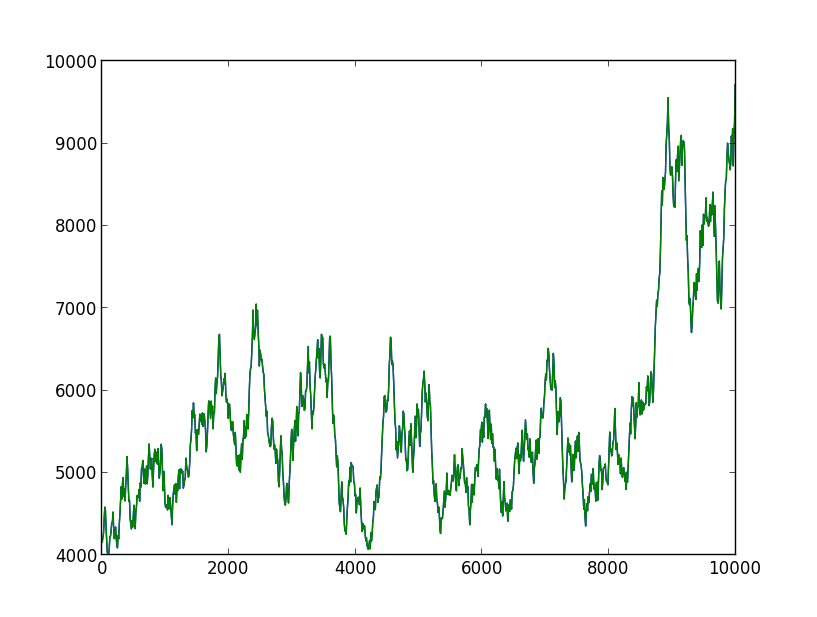
\includegraphics[width=0.5\textwidth]{images/query.png}
    \caption{Query plot}
    \label{fig:query}
\end{figure}

\begin{figure}[h!]
    \centering
    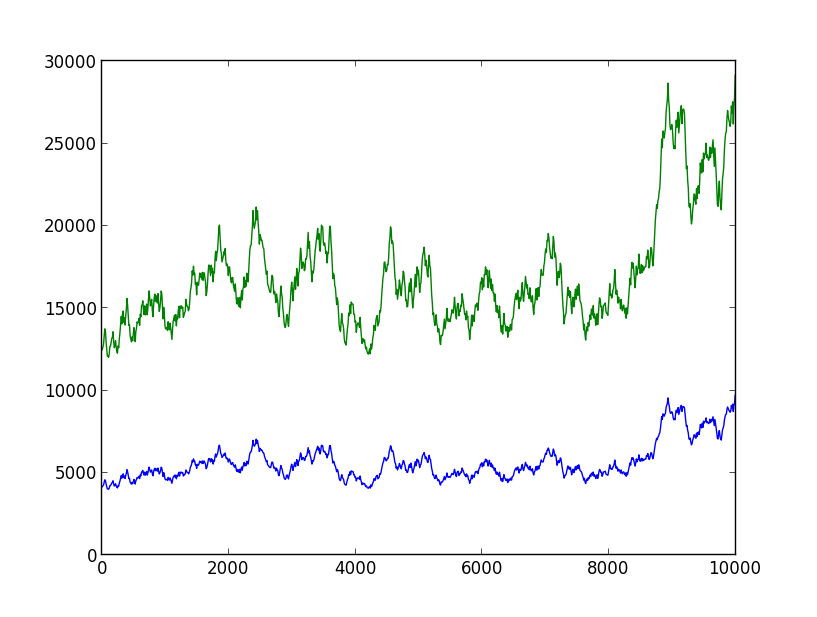
\includegraphics[width=0.5\textwidth]{images/mutant_1.png}
    \caption{First similar plot.  It is a scaling of the original plot by a factor of 3.}
    \label{fig:mutant_1}
\end{figure}

\begin{figure}[h!]
    \centering
    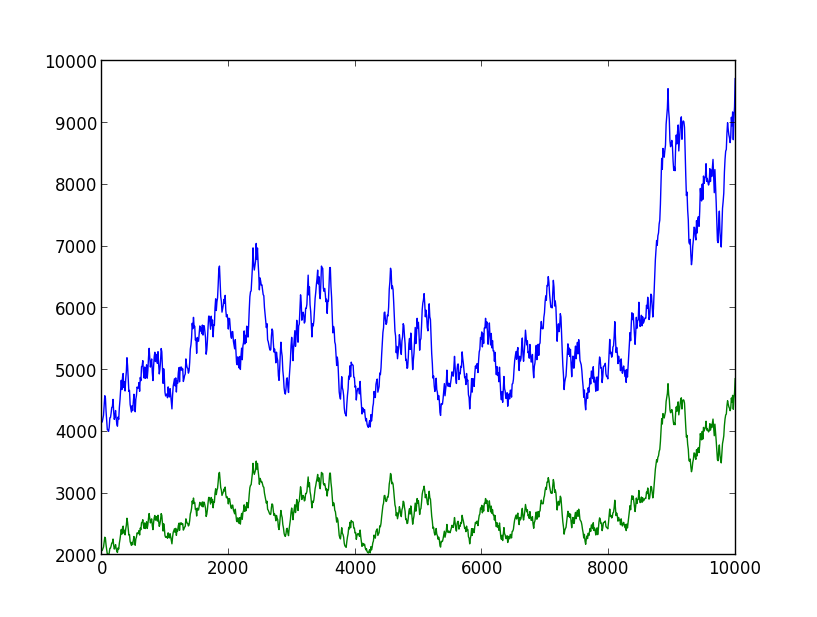
\includegraphics[width=0.5\textwidth]{images/mutant_2.png}
    \caption{Second similar plot.  It is a scaling of the original plot by a factor of 0.5.}
    \label{fig:mutant_2}
\end{figure}

\begin{figure}[h!]
    \centering
    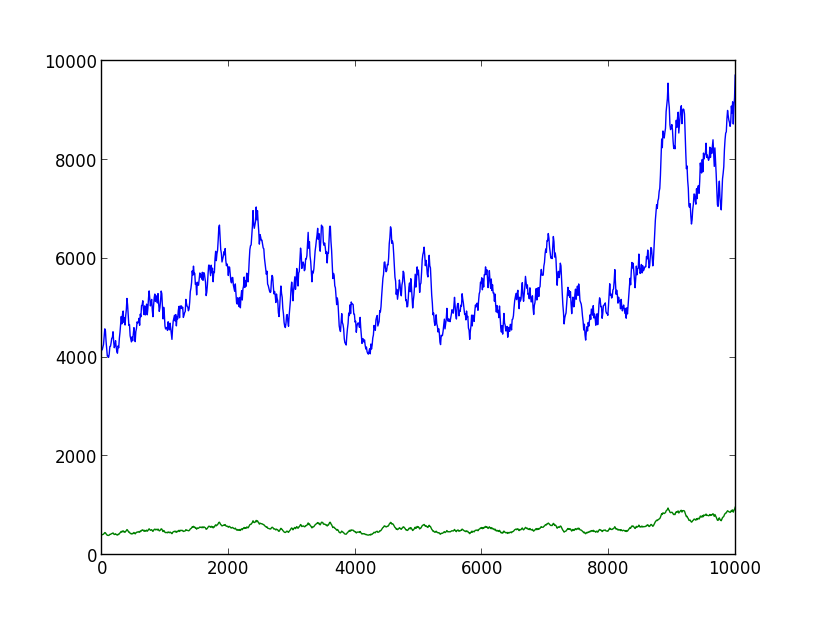
\includegraphics[width=0.5\textwidth]{images/mutant_3.png}
    \caption{Third similar plot.  It is a scaling of the original plot by a factor of 0.1.}
    \label{fig:mutant_3}
\end{figure}

\begin{figure}[h!]
    \centering
    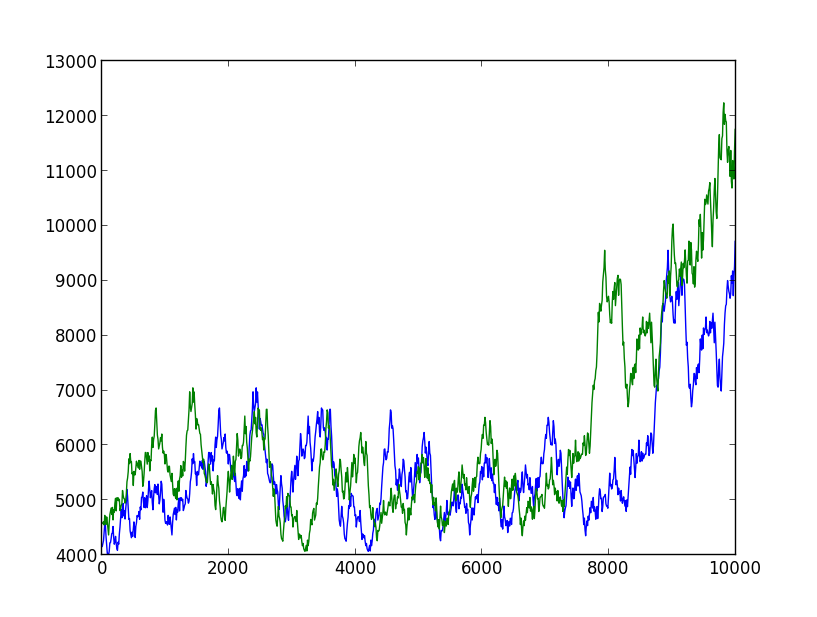
\includegraphics[width=0.5\textwidth]{images/mutant_4.png}
    \caption{Fourth similar plot.  The plot has been shifted left by 10\%.}
    \label{fig:mutant_4}
\end{figure}

\begin{figure}[h!]
    \centering
    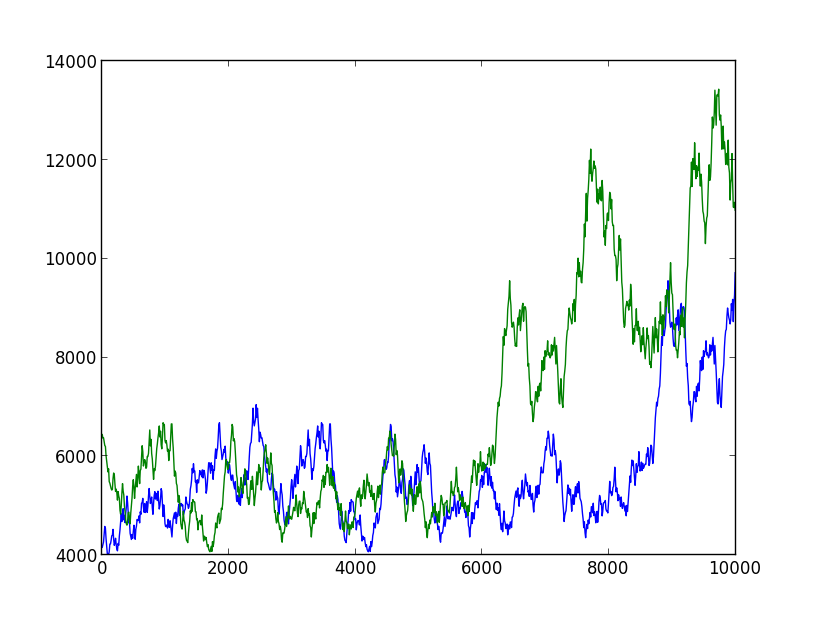
\includegraphics[width=0.5\textwidth]{images/mutant_5.png}
    \caption{Fifth similar plot.  The plot has been shifted left by 25\%.}
    \label{fig:mutant_5}
\end{figure}

\begin{figure}[h!]
    \centering
    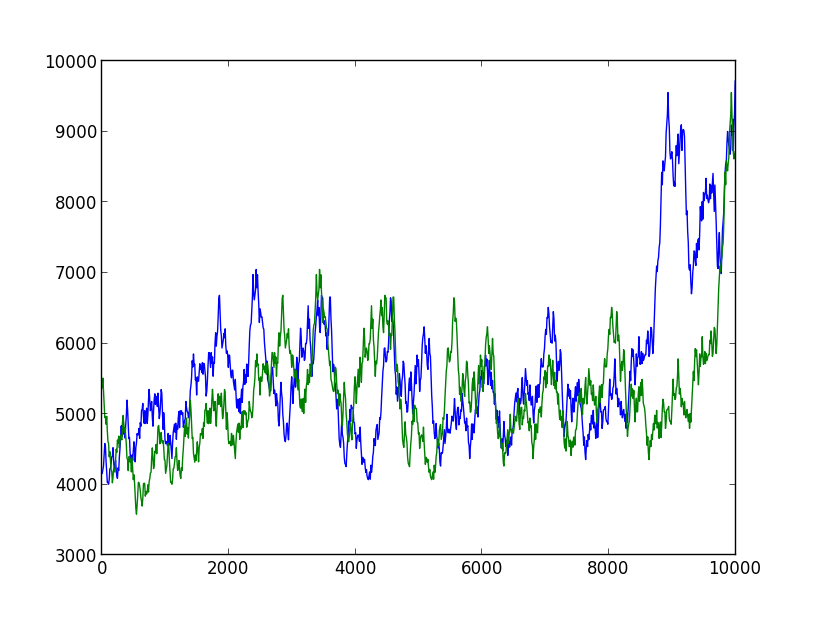
\includegraphics[width=0.5\textwidth]{images/mutant_6.png}
    \caption{Sixth similar plot.  The plot has been shifted right by 10\%.}
    \label{fig:mutant_6}
\end{figure}

\begin{figure}[h!]
    \centering
    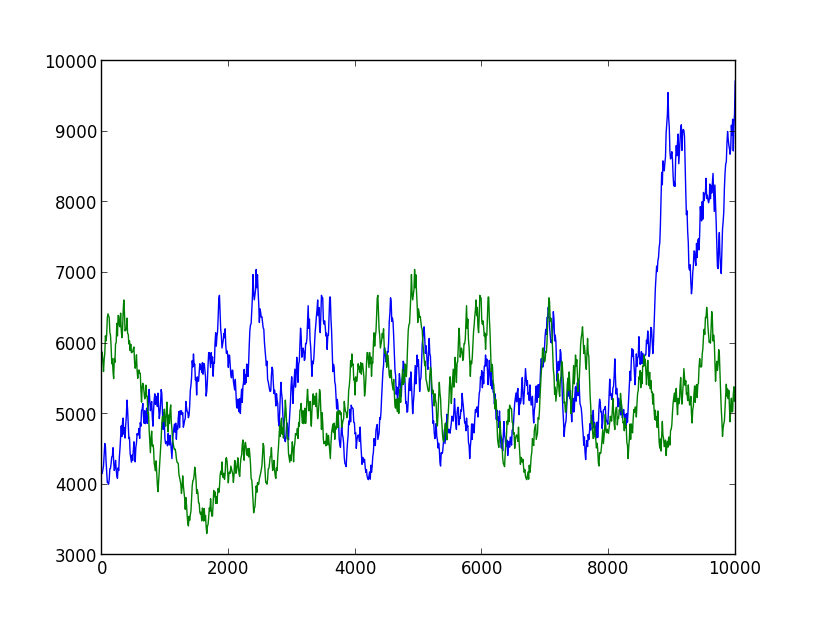
\includegraphics[width=0.5\textwidth]{images/mutant_7.png}
    \caption{Seventh similar plot.  The plot has been shifted right by 25\%.}
    \label{fig:mutant_7}
\end{figure}

\begin{figure}[h!]
    \centering
    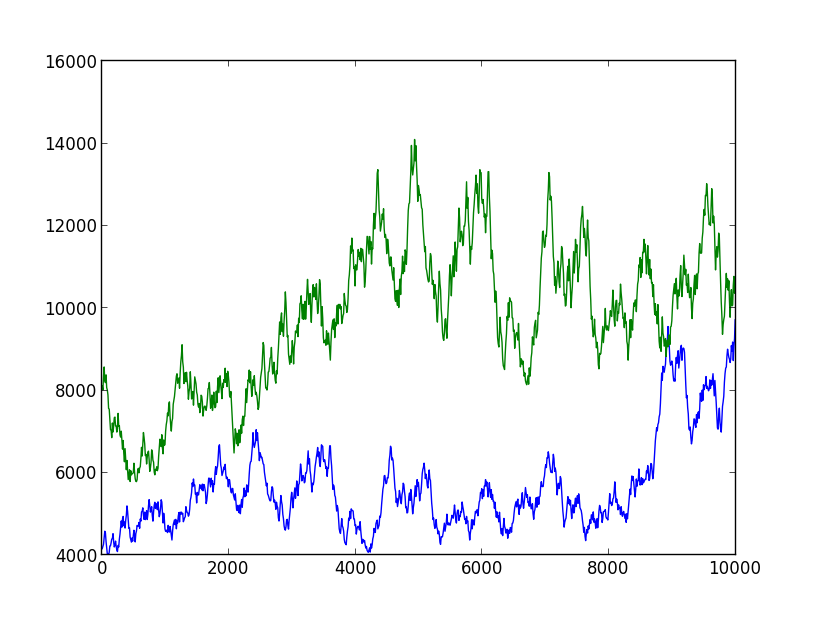
\includegraphics[width=0.5\textwidth]{images/mutant_8.png}
    \caption{Eighth similar plot.  The plot has been shifted right by 25\% and scaled by a factor of 2.}
    \label{fig:mutant_8}
\end{figure}

\begin{figure}[h!]
    \centering
    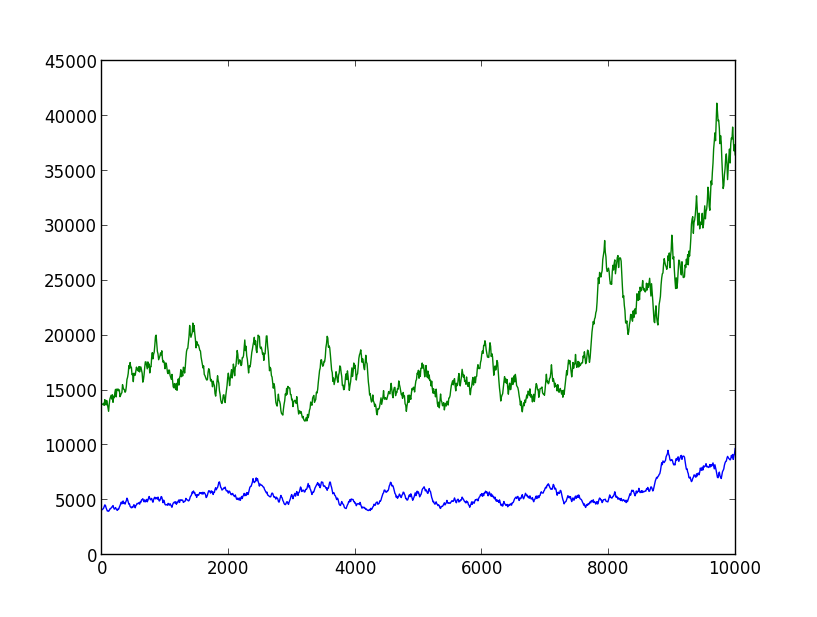
\includegraphics[width=0.5\textwidth]{images/mutant_9.png}
    \caption{Ninth similar plot.  The plot has been shifted left by 10\% and scaled by a factor of 3.}
    \label{fig:mutant_9}
\end{figure}

\begin{figure}[h!]
    \centering
    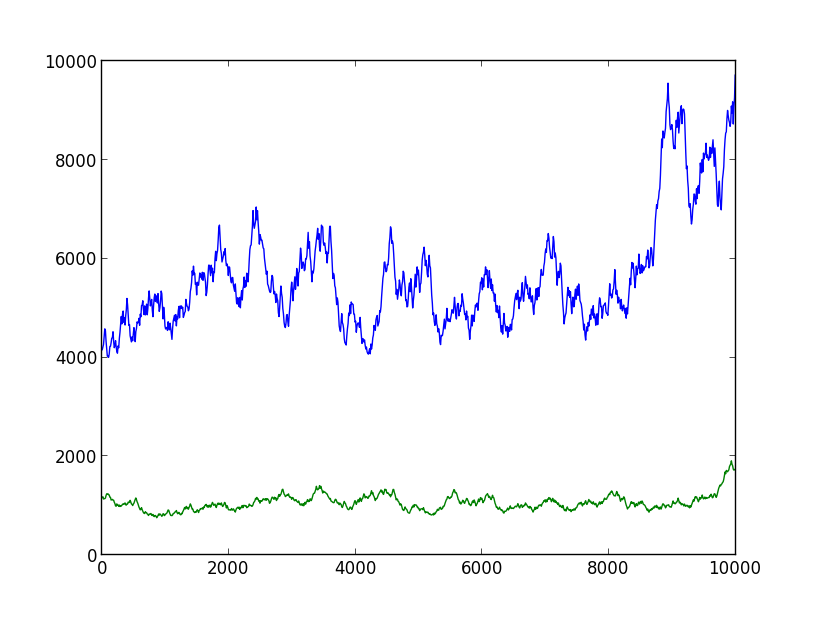
\includegraphics[width=0.5\textwidth]{images/mutant_10.png}
    \caption{Tenth similar plot.  The plot has been shifted right by 10\% and scaled by a factor of 0.2.}
    \label{fig:mutant_10}
\end{figure}

\clearpage

\section{Experiment 1 Graphs}
\label{sec:experiment1}

These are the plots for the results of Experiment 1 in Section~\ref{sec:search_eval}.  In all the graphs the query plot is the blue line and the plot determined to be similar is green.

\begin{figure}[h!]
    \centering
    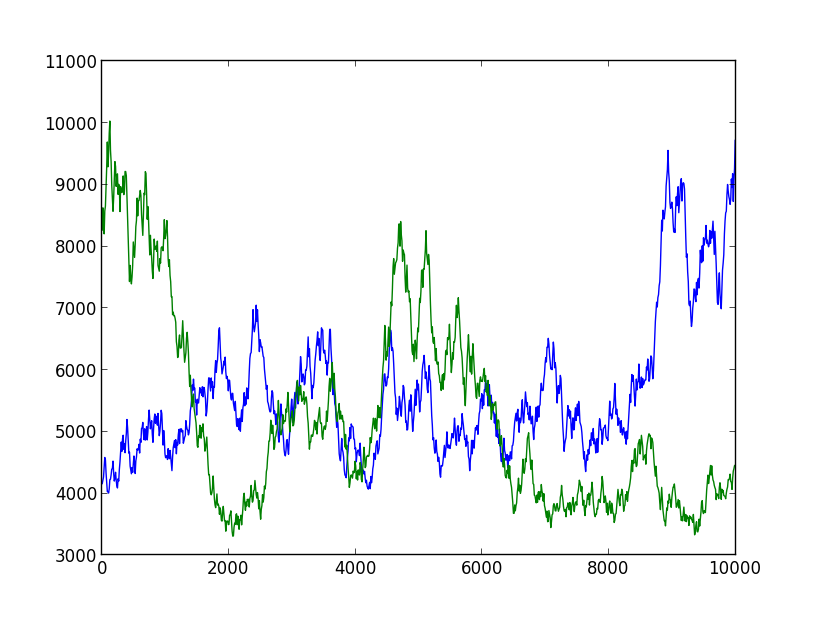
\includegraphics[width=0.5\textwidth]{images/256.png}
    \caption{First similar plot.  Line 256}
    \label{fig:ex1_1}
\end{figure}

\begin{figure}[h!]
    \centering
    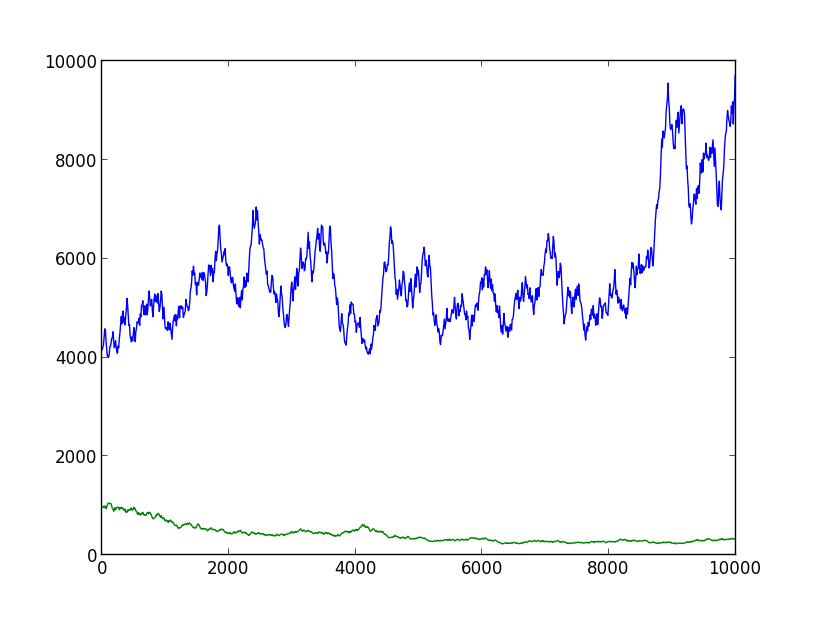
\includegraphics[width=0.5\textwidth]{images/7017.png}
    \caption{Second similar plot.  Line 7017}
    \label{fig:ex1_2}
\end{figure}

\begin{figure}[h!]
    \centering
    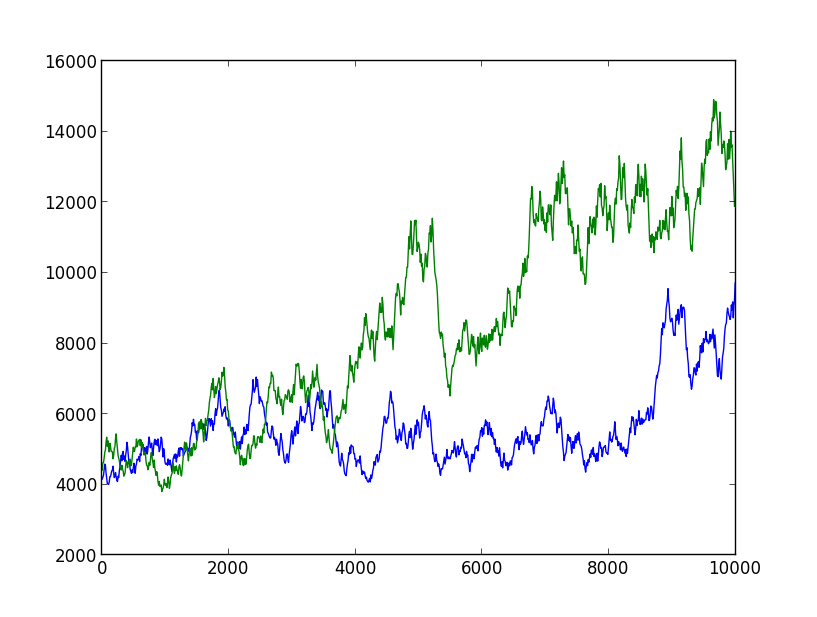
\includegraphics[width=0.5\textwidth]{images/8341.png}
    \caption{Third similar plot.  Line 8341}
    \label{fig:ex1_3}
\end{figure}

\begin{figure}[h!]
    \centering
    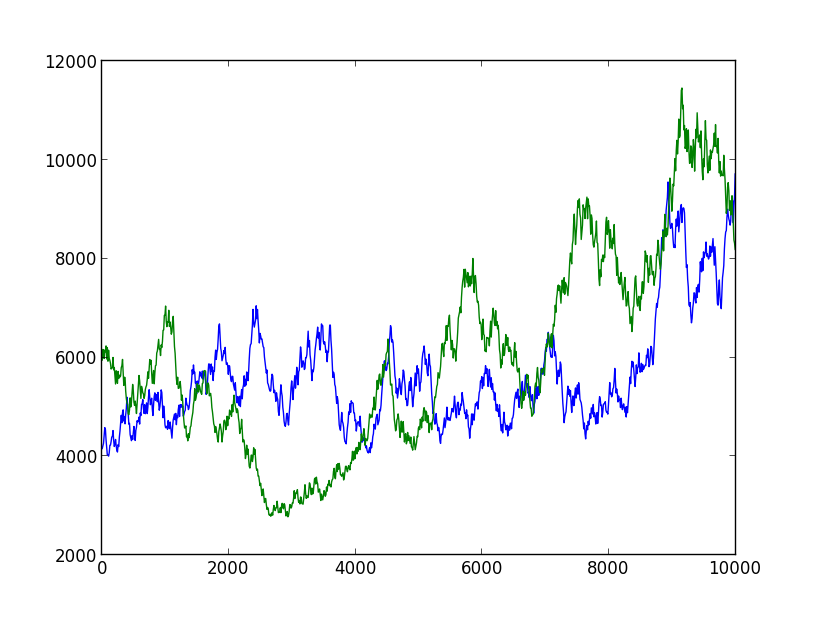
\includegraphics[width=0.5\textwidth]{images/1380.png}
    \caption{Fourth similar plot.  Line 1380}
    \label{fig:ex1_4}
\end{figure}

\begin{figure}[h!]
    \centering
    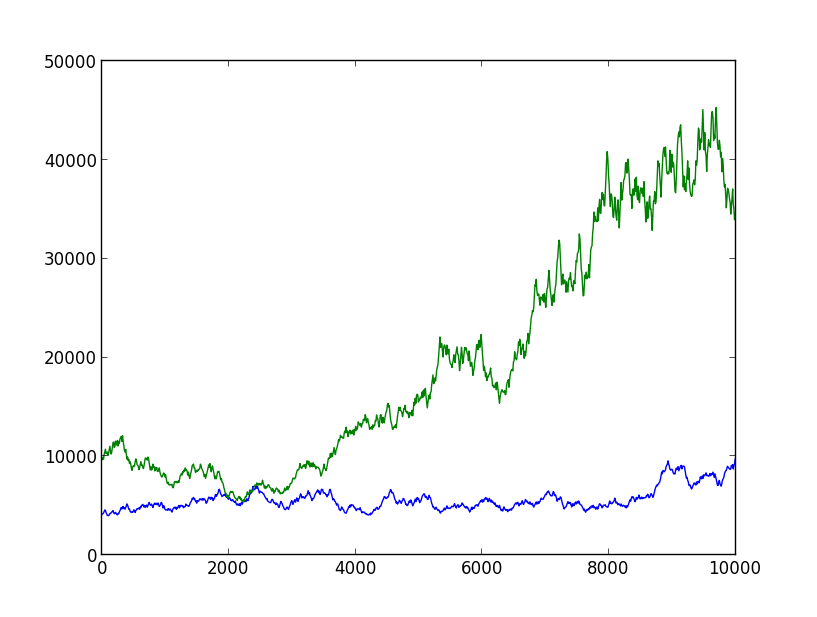
\includegraphics[width=0.5\textwidth]{images/4997.png}
    \caption{Fifth similar plot.  Line 4997}
    \label{fig:ex1_5}
\end{figure}

\begin{figure}[h!]
    \centering
    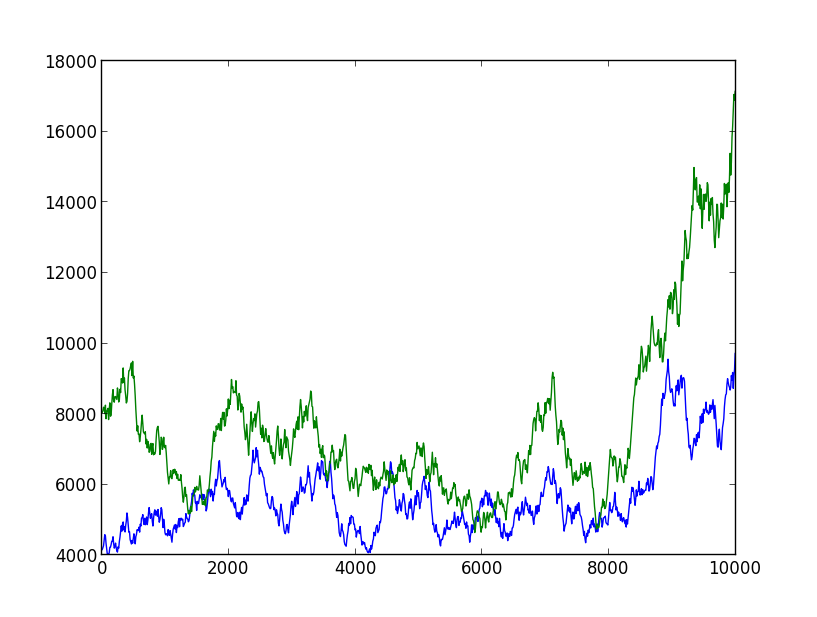
\includegraphics[width=0.5\textwidth]{images/5462.png}
    \caption{Sixth similar plot.  Line 5462}
    \label{fig:ex1_6}
\end{figure}

\begin{figure}[h!]
    \centering
    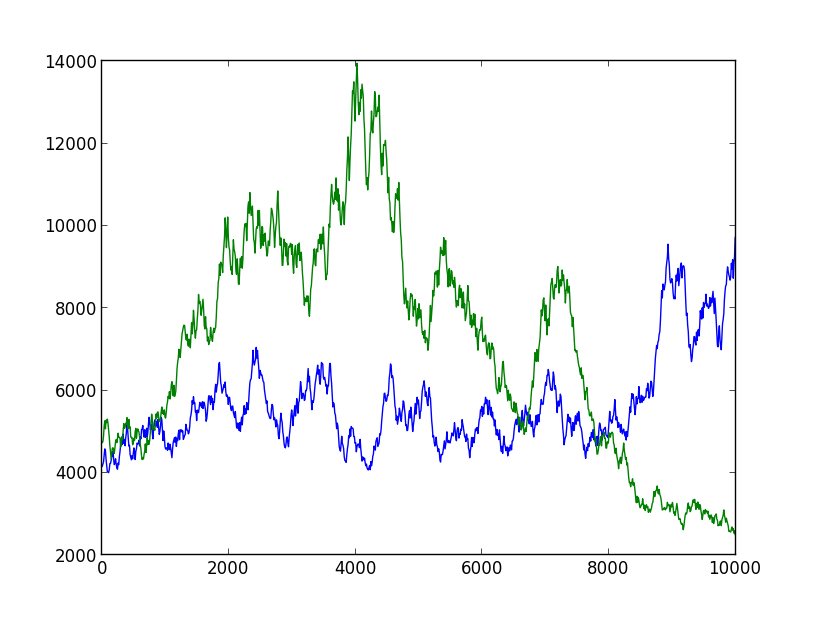
\includegraphics[width=0.5\textwidth]{images/6648.png}
    \caption{Seventh similar plot.  Line 6648}
    \label{fig:ex1_7}
\end{figure}

\begin{figure}[h!]
    \centering
    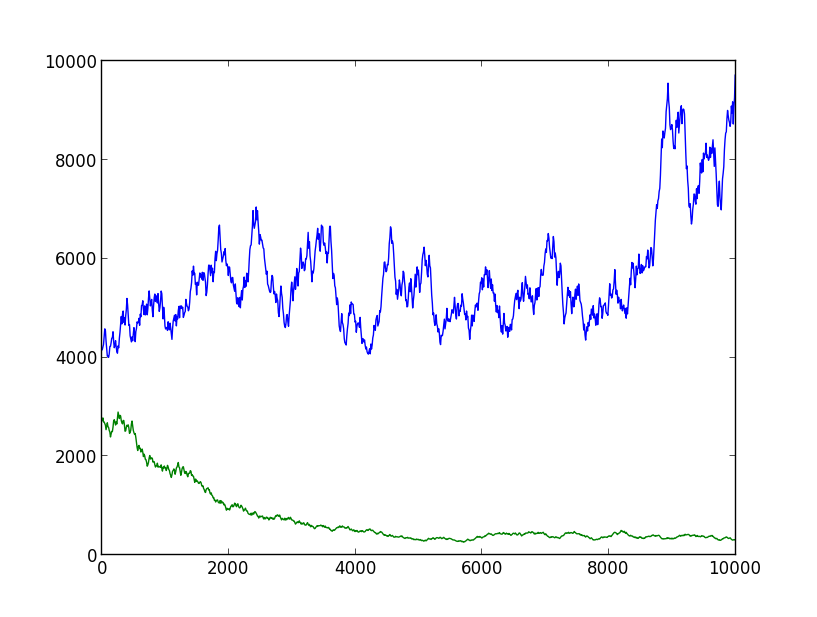
\includegraphics[width=0.5\textwidth]{images/2298.png}
    \caption{Eighth similar plot.  Line 2298}
    \label{fig:ex1_8}
\end{figure}

\begin{figure}[h!]
    \centering
    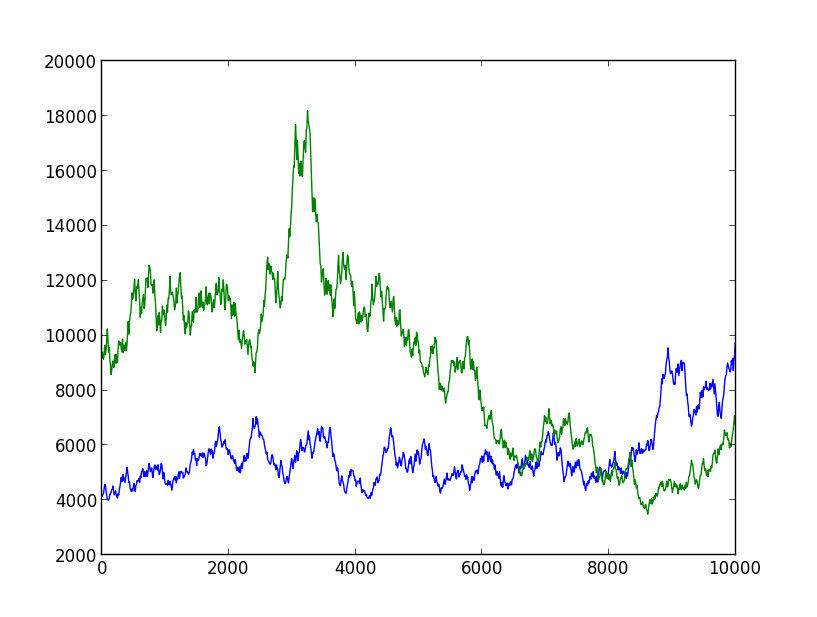
\includegraphics[width=0.5\textwidth]{images/595.png}
    \caption{Ninth similar plot.  Line 595}
    \label{fig:ex1_9}
\end{figure}

\begin{figure}[h!]
    \centering
    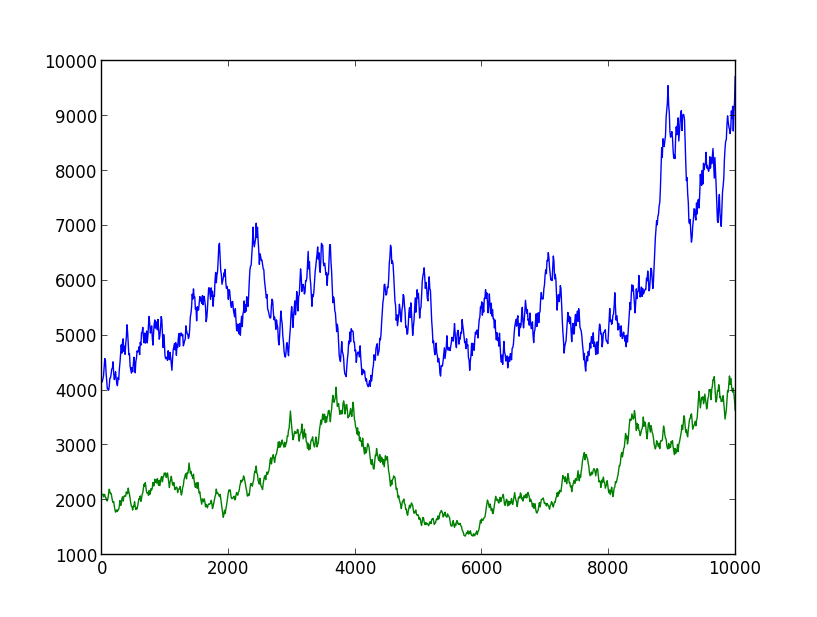
\includegraphics[width=0.5\textwidth]{images/190.png}
    \caption{Tenth similar plot.  Line 190}
    \label{fig:ex1_10}
\end{figure}
